\documentclass{beamer}

\title{The topology of Hilbert schemes of points on orbifolds}
\author{Paul Johnson}
\institute{Colorado State University \\
(from Columbia via Imperial) \\
\texttt{johnson@math.colostate.edu}
}
\date{June 7, 2013}



\usepackage{amsmath, amssymb}
\usepackage{tikz}
%\usepackage{mathpazo}
\newcommand{\Hilb}{\textrm{Hilb}}
\newcommand{\C}{\mathbb{C}}
\newcommand{\Z}{\mathbb{Z}}
\begin{document}
\newcommand{\stepright}[2]{%
\begin{scope}[xshift=#1cm,yshift=#2cm]
\clip (-.5, -.5)-- ++(1,1) -- ++(1,0) -- ++ (-1,-1) -- ++(-1,0);
\draw[cap=rect] (0,0)--(1,0);
\end{scope}
}
\newcommand{\stepdown}[2]{%
\begin{scope}[xshift=#1cm,yshift=#2cm]
\clip (-.5, -.5)-- ++(1,1) -- ++(0,-1) -- ++ (-1,-1) -- ++(0,1);
\draw[cap=rect] (0,0)--(0,-1);
\end{scope}
}

\begin{frame}[plain]
  \titlepage
\end{frame}

\begin{frame}{Outline}
\begin{block}{Goal:}
Understand Betti numbers of $\Hilb^n([\C^2/G])$
\end{block}

\begin{enumerate}
\item Betti numbers of $\Hilb^n(\C^2)$ 
\begin{itemize}\item Ellingsrud and Str\o mme \end{itemize}
\item Betti numbers of $\Hilb^n([\C^2/G])$ with $G\subset SL_2$ 
\begin{itemize}\item Gusein-Zade, Luengo, Melle-Hern\'andez \end{itemize}
\item Betti numbers of general case \begin{itemize} \item Me (some conjectures, some theorems) \end{itemize}
\end{enumerate}

\end{frame}
\begin{frame}{Basics of the Hilbert scheme of points on $\C^2$}
Let $R=\C[x,y]$.  Then:
$$\Hilb^n(\C^2):=\{\textrm{ideals }\mathcal{I}\subset R | \dim R/\mathcal{I}=n\}$$ 
\begin{itemize}
\item $\Hilb^n(\C^2)$ is smooth and connected of dimension $2n$.
\item Generically, $\mathcal{I}$ will be the ideal sheaf of $n$ distinct points in $\C^2$, so $\dim \Hilb^n(\C^2)=2n$.
\item When two or more points collide they become a ``fat point'' that remembers some information about how they collided.
\end{itemize}
\end{frame}

\begin{frame}{Warm-up: Euler-characteristic of $\Hilb^n(\C^2)$}
Before we find the Betti numbers let's find $\chi(\Hilb^n(\C^2))$:  

\begin{itemize}
\item The action of $(\C^*)^2$ on $\C^2$ induces a $(\C^*)^2$ action on $\Hilb^n(\C^2)$
\item The fixed points of the $(\C^*)^2$ action are the monomial ideals 
\item Since $\chi(\C^*)=\chi((\C^*)^2)=0$, the non-fixed orbits contribute nothing to the euler characteristic
\end{itemize}
So $\chi(\Hilb^n(\C^2))$ is the number ofmonomial ideals of length $n$.

\begin{block}{How many monomial ideals of length $n$ are there?}\end{block}



\end{frame}
\begin{frame}{Bijection between monomial ideals and partitions}
Monomials not in $\mathcal{I}$ are the cells of the partition.
Exterior corners of the partition are the generators of the monomial ideal.

\begin{center}
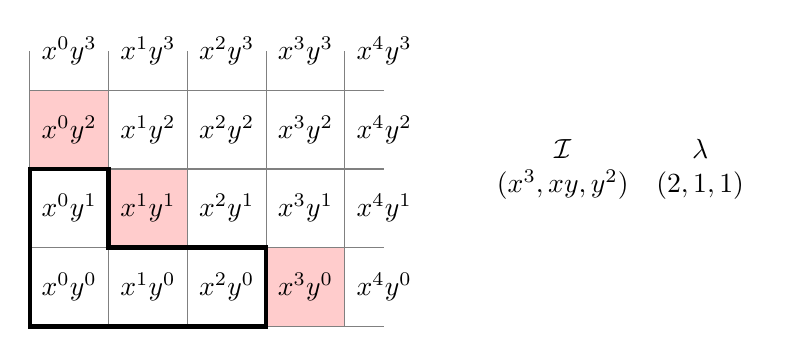
\begin{tikzpicture}
\draw[fill=red!20] (0,2) rectangle (1,3);
\draw[fill=red!20] (1,1) rectangle (2,2);
\draw[fill=red!20] (3,0) rectangle (4,1);


\draw[thin, gray] (0,0) grid (4.5,3.5);
\foreach \x in {0,...,4}
   \foreach \y in {0,...,3}
       \node at (\x+.5,\y+.5) {$x^\x y^\y$};
\draw[ultra thick, black] (0,0)--(0,2)--(1,2)--(1,1)--(3,1)--(3,0)--cycle;

\draw node at (7.5, 2) {$\begin{array}{cc} \mathcal{I} & \lambda \\ (x^3,xy,y^2) & (2,1,1) \end{array}$};
\end{tikzpicture}


\end{center}
So $\chi(\Hilb^n(\C^2))=p(n)$.
\end{frame}

\begin{frame}{Main motivating theorem}
Packaged into generating functions:
\begin{Theorem}[Warm-up]
$$\sum_{n\geq 0} \chi(\Hilb^n(\C^2))q^n=\sum_{n\geq0} p(n)q^n=\prod_{\ell\geq 1} \frac{1}{1-q^\ell}$$
\end{Theorem}

\begin{theorem}[Ellingsrud and Str\o mme, 1987]
$$\sum_{k,n \geq 0} b_k(\Hilb^n(\C^2))t^k q^n=\prod_{\ell=1}^\infty \frac{1}{1-t^{2\ell-2}q^\ell}$$
\end{theorem}
\begin{block}{Proof}
 Main tool is the \alert{Bia\l ynicki-Birula decomposition}
 \end{block}

\end{frame}

\begin{frame}{Bia\l ynicki-Birula decomposition $\approx$ Morse theory}
Suppose $X$ has a $\C^*$ action so that

\begin{enumerate}
\item $\lim_{\lambda\to 0} \lambda x$ exists for all $x\in X$
\item There are isolated fixed points
\end{enumerate}

Then we can compute the homology of $X$ by thinking of $x\mapsto\lambda x$ as $\lambda\to 0$ as a Morse flow, with the fixed points $p$ acting as the critical points.  

\begin{block}{What's the Morse index of a fixed point $p$?}
\end{block}
\end{frame}

\begin{frame}{Morse index = $2\dim T^-_pX$}

At each fixed point $p$, $T_pX$ is a $\C^*$ representation, and so splits into eigenspaces where $\lambda v=\lambda^a v$

\begin{description}
\item[$a=0$] Can't occur since fixed points are isolated
\item[$a>0$]  Flowing toward $p$
\item [$a<0$] Flowing away from $p$ 
\end{description}
$T^-_pX$ is the subspace where $a<0$.

\begin{Theorem}{Bia\l ynicki-Birula}
$$P_t(X)=\sum_{p\textrm{ fixed}} t^{\textrm{index}(p)}$$
\end{Theorem}
\begin{proof}
The differential is zero since all fixed points have even index.
\end{proof}
\end{frame}


\begin{frame}{Proof of Ellingsrud and Str\o mme}
\framesubtitle{Tangent spaces at fixed points}
\begin{Lemma}[Ellingsrud and Str\o mme, Cheah]
$$T_\lambda \Hilb^n(\C^2)=\sum_{\square\in\lambda} \left(x^{-\ell(\square)} y^{a(\square)+1}+x^{\ell(\square)+1}y^{-a(\square)}\right)$$
\end{Lemma}
Here $a(\square)$ and $\ell(\square)$ are the \alert{arm} and \alert{leg} of the square:
\begin{center}
\begin{tikzpicture}
\draw[thin, gray] (0,0) grid (1,3);
\draw[thin, gray] (1,0) grid (3,2);

\draw[thick] (0,0)--(0,3)--(1,3)--(1,2)--(3,2)--(3,1)--(4,1)--(4,0)--cycle;
\draw[fill=red!20] (1,0) rectangle (2,1);
\draw (1.5,1.5) node{$\clubsuit$};
\draw (2.5,.5) node{$\heartsuit$};
\draw (3.5,.5) node {$\heartsuit$};
\draw (6.5,1.5) node[align=left] {$a(\square)=\#\clubsuit=1$ \\ \\ $\ell(\square)=\#\heartsuit=2$};
\uncover<2>{
\begin{scope}[very thick, blue]
\draw(.5,.5) circle (.4);
\draw (.9, .5)--(2,.5);
\draw (4,1)--(2,.5)--(4,0);
\draw (1,2)--(1.5,.5)--(1,-1);}
\end{scope}
\end{tikzpicture}

\end{center}
\end{frame}

\begin{frame}{Proof of Ellingsrud and Str\o mme}
\framesubtitle{Putting everything together}
\begin{block}{Pick a $\C^*\subset (\C^*)^2$}
Use the $\C^*$ acting by $$\lambda\cdot(x,y)=(\lambda^\epsilon x, \lambda y)$$
With $ 0<\epsilon<<1$.
\end{block}

\begin{itemize}
\item $x^{-\ell(\square)} y^{a(\square)+1}\mapsto \lambda^{1+a(\square)-\epsilon\ell(\square)}$ is always positive
\item $x^{\ell(\square)+1}y^{-a(\square)}\mapsto \lambda^{-a(\square)+\epsilon(1+\ell(\square))}$ negative when $a(\square)>0$.
\end{itemize}
\begin{center}
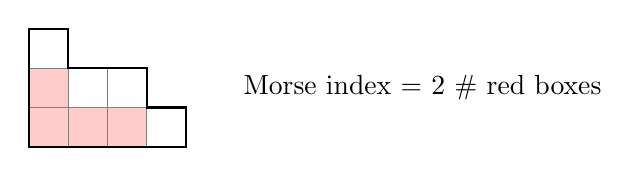
\begin{tikzpicture}[scale=.5]
\draw[fill=red!20] (0,0) rectangle (1,2);
\draw[fill=red!20] (0,0) rectangle (3,1);


\draw[thin, gray] (0,0) grid (1,3);
\draw[thin, gray] (1,0) grid (3,2);

\draw[thick] (0,0)--(0,3)--(1,3)--(1,2)--(3,2)--(3,1)--(4,1)--(4,0)--cycle;

\draw (10,1.5) node[align=left] {Morse index = 2 \# red boxes};
\end{tikzpicture}
\end{center}
\end{frame}


\begin{frame}{Proof of Ellingsrud and Str\o mme}
\framesubtitle{Putting everything together}

\begin{center}
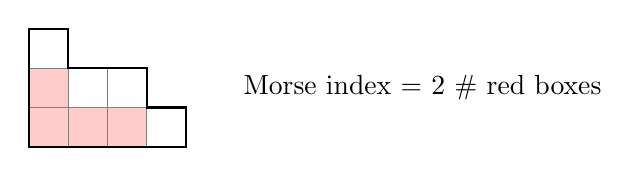
\begin{tikzpicture}[scale=.5]
\draw[fill=red!20] (0,0) rectangle (1,2);
\draw[fill=red!20] (0,0) rectangle (3,1);


\draw[thin, gray] (0,0) grid (1,3);
\draw[thin, gray] (1,0) grid (3,2);

\draw[thick] (0,0)--(0,3)--(1,3)--(1,2)--(3,2)--(3,1)--(4,1)--(4,0)--cycle;

\draw (10,1.5) node[align=left] {Morse index = 2 \# red boxes};
\end{tikzpicture}
\end{center}

A column of height $h$ contributes $q^ht^{2h-2}$
$$\sum_{k,n \geq 0} b_k(\Hilb^n(\C^2))t^k q^n=\prod_{\ell=1}^\infty \frac{1}{1-t^{2\ell-2}q^\ell}\qed$$


\end{frame}

\begin{frame}{Building on Ellingsrud-Str\o mme}

\begin{Theorem}[G\"ottsche, 1990]
Let $S$ be a smooth quasi-projective surface with Betti numbers $b_i$.  Let $S^{(n)}=\Hilb^n(S)$.  Then
$$\sum b_k(S^{(n)})t^k q^n=\prod_{\ell\geq 1} \frac{(1+t^{2\ell-1}q^\ell)^{b_1}(1+t^{2\ell+1}q^\ell)^{b_3}}{(1-t^{2\ell-2}q^\ell)^{b_0}(1-t^{2\ell}q^\ell)^{b_2}(1-t^{2\ell+2}q^\ell)^{b_4}}$$

\end{Theorem}
\begin{proof} Ellingsrud and Str\o mme + Weil Conjectures
\end{proof}
\begin{Theorem}[Nakajima, Grojnowski]
$\bigoplus H_k(\Hilb^n(S))$ is a highest weight representation for a Heisenberg algebra generated by $H^*(S)$.

\end{Theorem}

\end{frame}

\begin{frame}{Orbifold Hilbert Schemes are fixed point sets}


\begin{eqnarray*}
\Hilb^n([\C^2/G])&:=&\{\textrm{$G$-equivariant ideals } \mathcal{I}\subset R\} \\
&=&\Hilb^n(\C^2)^G\subset \Hilb^n(\C^2)
\end{eqnarray*}
\begin{itemize}
\item As a fixed point set in a smooth variety, we see $\Hilb^n([\C^2/G])$ is smooth.
\item Not connected.  One discrete invariant: $R/\mathcal{I}$ isn't just a vector space, it's a representation of $G$.  
\end{itemize}

For $v\in K_0(G)$, let $\Hilb^v_G$ denote the component where $R/\mathcal{I}=v$.

\end{frame}

\begin{frame}{Colo(u)red boxes}
Restrict to $G=\Z/r\Z$, with action $(\exp(2\pi i /r),\exp(2\pi i m/r))$.
For a monomial ideal, keeping track of $K_0(G)$ class is counting colored boxes:
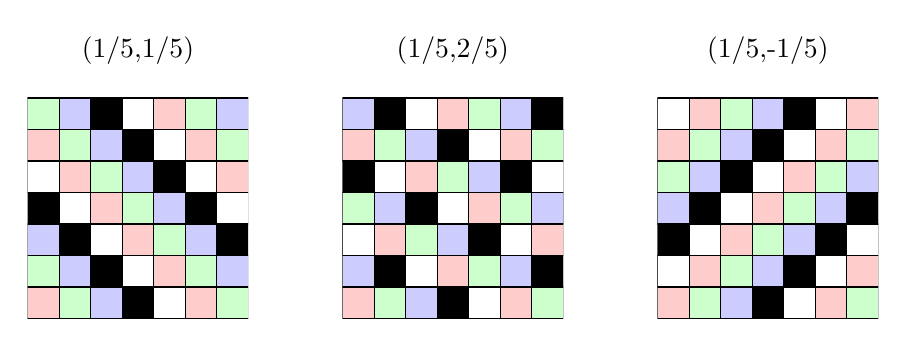
\begin{tikzpicture}[scale=.4]
\begin{scope}
\draw (3.5,8.5) node{(1/5,1/5)};
       \clip (0,0) rectangle (7,7);
\foreach \x in {0,...,6}{%
    \foreach \y in {-2,...,2}{%
       \draw[fill=red!20]  (\x, -\x+5*\y) rectangle (\x+1, -\x+5*\y+1); 
       \draw[fill=green!20]  (\x, -\x+5*\y+1) rectangle (\x+1, -\x+5*\y+2); 
       \draw[fill=blue!20]  (\x, -\x+5*\y+2) rectangle (\x+1, -\x+5*\y+3); 
       \draw[fill=black]  (\x, -\x+5*\y+3) rectangle (\x+1, -\x+5*\y+4);
        \draw  (\x, -\x+5*\y+4) rectangle (\x+1, -\x+5*\y+5); 
}}
\end{scope}     

\begin{scope}[xshift=10cm]
\draw (3.5,8.5) node{(1/5,2/5)};
\begin{scope}[xscale=-1, rotate=90]
       \clip (0,0) rectangle (7,7);
\foreach \x in {0,...,6}{%
    \foreach \y in {-4,...,2}{%
       \draw[fill=red!20]  (\x, 3*\x+5*\y) rectangle (\x+1, 3*\x+5*\y+1); 
       \draw[fill=green!20]  (\x, 3*\x+5*\y+1) rectangle (\x+1, 3*\x+5*\y+2); 
       \draw[fill=blue!20]  (\x, 3*\x+5*\y+2) rectangle (\x+1, 3*\x+5*\y+3); 
       \draw[fill=black]  (\x, 3*\x+5*\y+3) rectangle (\x+1, 3*\x+5*\y+4);
        \draw  (\x, 3*\x+5*\y+4) rectangle (\x+1, 3*\x+5*\y+5); 
}}
\end{scope}
\end{scope}     

\begin{scope}[xshift=20cm]
\draw (3.5,8.5) node{(1/5,-1/5)};
\begin{scope}[xscale=-1, rotate=90]
       \clip (0,0) rectangle (7,7);
\foreach \x in {0,...,6}{%
    \foreach \y in {-2,...,2}{%
       \draw[fill=red!20]  (\x, \x+5*\y) rectangle (\x+1, \x+5*\y+1); 
       \draw[fill=green!20]  (\x, \x+5*\y+1) rectangle (\x+1, \x+5*\y+2); 
       \draw[fill=blue!20]  (\x, \x+5*\y+2) rectangle (\x+1, \x+5*\y+3); 
       \draw[fill=black]  (\x, \x+5*\y+3) rectangle (\x+1, \x+5*\y+4);
        \draw  (\x, \x+5*\y+4) rectangle (\x+1, \x+5*\y+5); 
}}
\end{scope}     
\end{scope}

\end{tikzpicture}

\end{frame}




\begin{frame}{Special McKay Correspondence}
When $S$ is smooth, $\Hilb^1(S)=S$,  but $\Hilb^1([\C^2/G])=\textrm{point}$.

The ideal sheaf of a smooth point on $[\C^2/G]$ corresponds to the regular representation of $G$.

\begin{theorem}
$\Hilb_G^G([\C^2/G])$ is the minimal resolution of $\C^2/G$.
\end{theorem}

\begin{itemize}
\item The minimal resolution of $\C^2/G$ is a chain of $c$ rational curves
\item When $G\subset SL_2, c=|G|-1$, and so $\chi(\Hilb_G^G([\C^2/G])=|G|$
\item Otherwise, $c<|G|-1$, and $\Hilb_G^G([\C^2/G])$ only sees some of $K_0(G)$
\end{itemize}





%Rather than just increasing the length of the partition, it makes sense to study what happens as we add more copies of $G$.





\end{frame}


\begin{frame}{Generating series for orbifold Hilbert schemes}
Restrict to $G=\Z/r\Z$, with action $(\exp(2\pi i /r),\exp(2\pi i m/r))$.
\begin{block}{Disconnected generating series}
$$\mathcal{DH}_{m/r}:=\sum_{n,k\geq 0 } b_k(\Hilb^n([\C^2/G])) t^kq^n$$
\end{block}
Call an element $\delta\in K_0(G)$ small if $\Hilb^\delta_G$ is nonempty but compact; equivalently, if it is nonempty but $\Hilb^{\delta-G}_G$ is empty.

\begin{block}{Connected generating series}
For $\delta\in K_0(G)$ small, define 
$$\mathcal{CH}^\delta_{m/r}:=\sum_{n,k\geq 0} b_k(\Hilb^{\delta+nG}([\C^2/G]))t^kq^n$$
\end{block}
\end{frame}

\begin{frame}{How to calculate these Betti numbers?}
Follow proof of Ellingsrud-Str\o mme, but the index of each partition will change:

\begin{Lemma}[Ellingsrud and Str\o mme, Cheah]
$$T_\lambda \Hilb^n(\C^2)=\sum_{\square\in\lambda} \left(x^{-\ell(\square)} y^{a(\square)+1}+x^{\ell(\square)+1}y^{-a(\square)}\right)$$
\end{Lemma}

A tangent direction only contributes to $T_\lambda \Hilb^n([\C^2/G])$ if it is $G$-invariant.  
\begin{example}[Balanced $\Z_r$ action]
A generator acts as $(-1/r,1/r)$, so we need $\ell(\square)+a(\square)+1$ to be divisible by $r$
\end{example}

\end{frame}

\begin{frame}
\begin{Theorem}[Gusein-Zade, Luengo, Melle-Hern\'andez]
$$\mathcal{H}^0_{-1/r}=\prod_{\ell\geq 1}\frac{1}{1-t^{2\ell-2}q^\ell}\frac{1}{(1-t^{2\ell}q^\ell)^{r-1}}$$
$$\mathcal{H}_{-1/r}=\prod_{\ell\geq 1} \frac{(1-q^{r\ell})^r}{1-q^\ell}\frac{1}{1-t^{2\ell-2}q^{r\ell}}\frac{1}{(1-t^{2\ell}q^{r\ell})^{r-1}}$$
\end{Theorem}
\begin{proof}
Cores and quotients of partitions.
\end{proof}
 $\Hilb^{\delta+nG}_{-1/r}$ are Nakajima quiver varieties, and are all diffeomorphic to $\Hilb^{nG}_{-1/r}$.
\begin{block}{What about the unbalanced case?}\end{block}
\end{frame}

\begin{frame}{Start of unbalanced case}
Recall $(a;x)_\infty:=\prod_{\ell\geq 0} (1-ax^\ell)$.
\begin{example}[G\"ottsche]
$$\sum_{n\geq 0} b_k(\Hilb^n(S))t^kq^n=
\frac{1}{(q;qt^2)_\infty^{b_0}}\frac{1}{(qt^2;qt^2)_\infty^{b_2}}\frac{1}{(qt^4;qt^2)_\infty^{b_4}}$$
\end{example}
\begin{block}{Conjecture (Gusein-Zade, Luengo, Melle-Hern\'andez)]}

$$\mathcal{H}_{1/3}=\frac{1}{(q;t^2q^3)_\infty}\frac{1}{(q^2t^2;t^2q^3)_\infty}\frac{1}{(q^3;t^2q^3)_\infty}$$
\end{block}
\begin{block}{Why stop there?} 
\end{block}
\end{frame}


\begin{frame}{Main conjecture on disconnected series}
 It seems if $G\cap SL_2=\emptyset$ then
$$\mathcal{H}_{G}=\prod_{h=1}^r \frac{1}{(q^h t^{\epsilon(h)}; q^r t^2)_\infty}$$
with $\epsilon(h)$ either 2 or 0.

\begin{block}{Conjecture (Johnson)}
If $g\in G$ acts on $\C^2$ as $(\exp(2\pi i a/r),\exp(2\pi i b/r)$, let $AF(g)$ and $AI(g)$ denote the fractional and integral parts of $a/r+b/r$.
Let $k=|G\cap SL_2|$.

$$\mathcal{H}_G(q,t)= \frac{(q^k;q^k)^k_\infty}{(q,q)_\infty} \prod_{g\in G}\frac{1}{q^{r(1-AF(g)} t^{2AI(g)},q^rt^2)_\infty}$$

\end{block}

\end{frame}

\begin{frame}{Results on connected Hilbert schemes}
\begin{Theorem}[Johnson]
$P_t(\Hilb^{\delta+nG}_G)$ stabilizes to $1/(t,t)_\infty^{|G|}$
\end{Theorem}
Note that the right hand side is independent of $m$ and $\delta$.

\begin{block}{Conjecture (Johnson)}
Let $c$ be the number of rational curves in the minimal resolution of $\C^2/G$.  Then
$$\mathcal{H}^\delta_G\cdot(q,qt^2)_\infty\cdot (qt^2,qt^2)_\infty^c$$
has positive coefficients.
\end{block}
Though total homology sees all of $K_0(G)$, only get a Heisenberg action for the minimal resolution.

\end{frame}

\end{document}